% !TeX spellcheck = en_US
\section{Material and Methods}
    
    %------------------------------%
    %& General approach
    %------------------------------%
    % We generated 180 data sets with varying sample sizes and abundance response shapes. 
    % %
    % Using these data sets, we tested the ability of four multivariate statistical techniques to differentiate between causal and noise variables.  

	%------------------------------%
	%&		Simulations 			
	%------------------------------%

	\subsection{Data Generation}
		Species abundances were simulated as counts, a common abundance measure in ecology \citep{Warton2008}. 
		%
		Abundances were stored in $\mathbf{Y}$, an $N \times S$ matrix of responses, in this case, the abundances of $S$ species, $ s= 1\ ...\ S$, at $N$ sites, $ n = 1\ ...\ N$.
		%
		The species in $\mathbf{Y}$ responded to  environmental variable $x_m$ with one of three different response types: unimodal (\textit{U}), linear (\textit{L}) or bimodal (\textit{B}), as shown in Figure \ref{fig:bivariateExample}.
        %
		These environmental variables are stored in $\mathbf{X}$ an $N \times M$ matrix with $M$ environmental variables, $m = 1\ ... \ M$. 
	    %
	    The simulation process is visualized in Figure \ref{fig:flowchart_simulation}. 
	    
	    
	%--------------------------------%
	%&		Figure: 3d Response shapes	
	%--------------------------------%
		\begin{figure}[ht]
			
			\begin{center}
			    
			    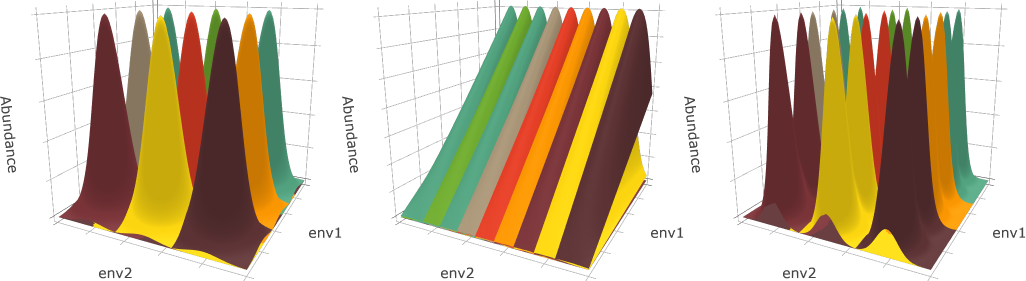
\includegraphics[width = 1\linewidth]{figures/Communities_trimmed_appended.png}     
			   	\caption{
			                Simulated abundance responses along two causal variables (\textit{env1} and \textit{env2}). 
                			%
                            Response combinations are: unimodal-unimodal (left), unimodal-linear (middle) and unimodal-bimodal (right). 
                			%
                			The vertical axis indicates abundance. 
                			%
                			The different colors represent different species.
                			%
                			All the examples show the unsampled abundance matrix
                			$\mathbf{Y_{Large}}$.
			            }
			\label{fig:bivariateExample} 
			\end{center}
			

		\end{figure}
        
		%------------------------------%
		%&		Environmental Gradients				
		%------------------------------%        
        %
		We simulated abundances along two environmental gradients \textit{env1} and \textit{env2}, which henceforth will be referred to as causal variables to differentiate them from the noise variables.  
		%
        Both causal variables consist of the natural numbers from 1 to 100. 
        %
        Each possible combination of the two is a site, i.e. the total number of sites N = 10.000.
		%
		$\mathbf{Y_{Large}}$ holds the simulated abundances for all 10.000 sites.
	    %
	    This data set is larger than most ecological field data sets and fitting models to it would have required considerable computation time.
	    %
	    Therefore, we sampled from $\mathbf{Y_{Large}}$ with six different samples sizes (25, 100, 225, 400, 625, and 900) to obtain $\mathbf{Y_{Sample}}$.
        %
        Depending on the sample size $n$, a set number ($\sqrt{n}$) of sampling locations per causal variable were chosen. 
        %
        These locations always included the variable's minimum and maximum values (i.e. 1 and 100), between those, the locations were equidistantly distributed.
		%
		The abundances of all species at all combinations of sampling locations constitute $\mathbf{Y_{Sample}}$.
		%
		All species show the same response type towards each causal variable, but response types can differ between variables (Figure \ref{fig:bivariateExample}). 
	    %
		This setup allows for six communities each with a different combination of response types, including those with identical response types to both variables (Figure \ref{fig:flowchart_simulation}).  
		%
		The communities are labeled with their abbreviated response types, e.g. \textit{LB} for a community  in which species' abundances respond linearly to the first and bimodally to the second causal variable (Figure \ref{fig:bivariateExample}c). \\
		%------------------------------%
		%&		Responses				
		%------------------------------%
		Unimodal responses were simulated using the Gaussian response model \citep{GauchJr1972} expanded to multiple dimensions (Eqn. \ref{eq:GaussianResponseModel}).
		%
		\begin{equation} \label{eq:GaussianResponseModel}
					y_{s, n} = \prod_{m}^{M_{uni}} c_{s,m} \times exp\bigg(-\frac{(x_{m,n} - u_{s,m})^2}{2t^2_{s,m}}\bigg)		
		\end{equation}
		%	
    	where $u_{s,m}$ is the position of the optimum (i.e. the point with the highest abundance) of species $s$ along the environmental variable $m$, $t_{s, m}$ is the tolerance of species $s$ toward that variable and determines the width of the unimodal curve and $c_{s,m}$ is the maximal abundance of species $s$ on environmental variable $m$. 
		%
		$M_{uni}$ is the number of unimodal environmental variables. 
		%
% 		Note that all environmental variables themselves are actually linear and only the response toward them is variable. 
% 		%
% 		To improve readability though, we will refer to environmental variables in the manner that species respond to them. \\
		%
		Linear responses were simulated by multiplying the environmental variables with a coefficient $\beta$ (Eqn. 2).
		%
		\begin{equation}
		 				y_{s,n} = \prod_{m}^{M_{lin}} x_{m,n} \times \beta_{s,m}
		\end{equation}
		%
		Bimodal responses were simulated by adding two unimodal models with different optima $u_{s,m}$.\\
		%
		This way we obtained $M = 2$ abundance values $y_{m,s,n}$ per species and site. 
		%
		To obtain a single abundance $y_{s,n}$ for each species at each site, we multiplied the abundances of each environmental variables.
		%
		By multiplying instead of adding the abundance values, we ensured that a species is absent from sites where its abundance drops to zero for one of the gradients, i.e. is outside of its niche. 

	%------------------------------%
	%&		Figure: Flowchart 	
	%------------------------------%
		
		\begin{figure}[ht]
			\centering
			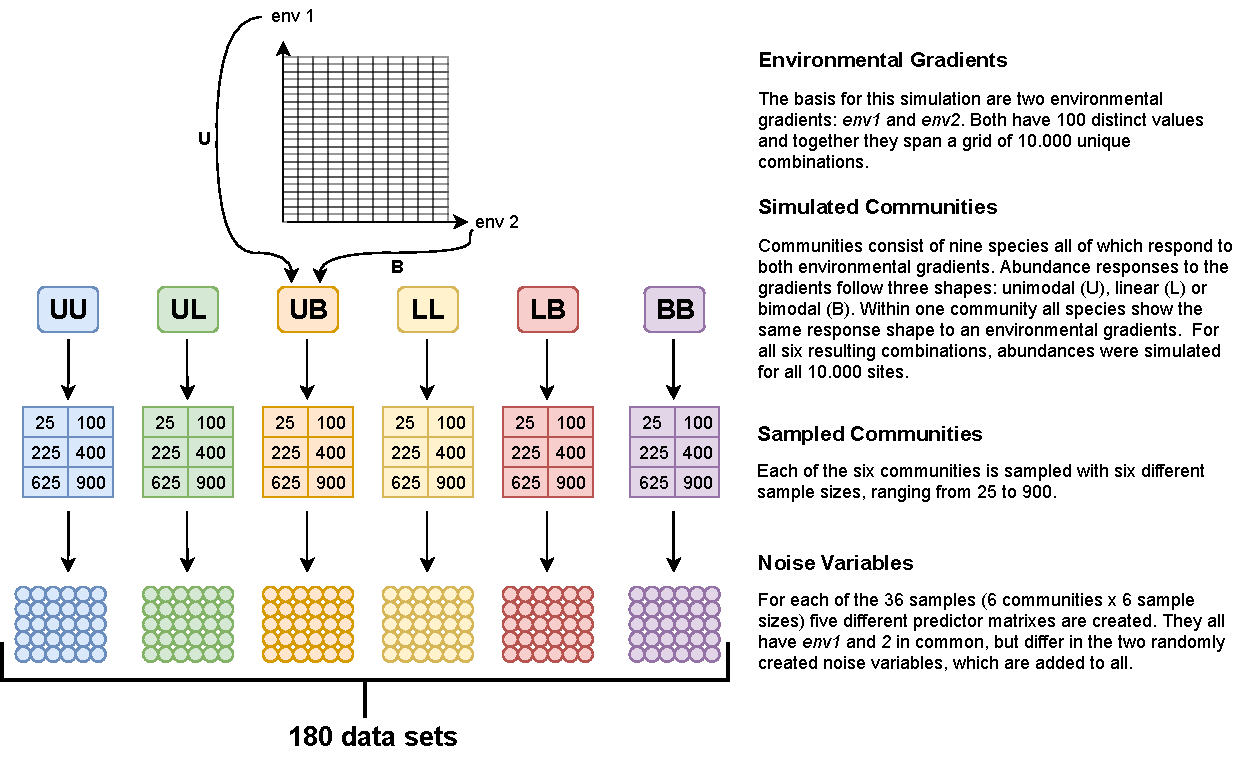
\includegraphics[width=1\linewidth]{figures/190917_MTP_MM_FLOWCHART.pdf}
			\caption{
			        Flowchart of the community simulations. 
			        %
			        The environmental space is comprised out of two variables (\textit{env1} and \textit{env2}) and 10.000 unique sites.
			        %
			        At each site the abundances of nine species are simulated. 
			        %
			        Abundance responses to environmental gradients display three shapes:
			        unimodal (U), linear (L) and bimodal (B). 
			         %
			         All nine species of one community show the same response shape (with varying parameters) to one gradient, but response shapes can differ between gradients. 
			         %
			         All six possible combination of response shapes are sampled with six different sample sizes spanning from 25 to 900.
			        %
                    Before these data are analysed two noise variables are added two $\mathbf{X}$ .
                    %
                    For each response shape - sample size combination, five different pairs of noise variables are appended to $\mathbf{X}$. 
			        }
			\label{fig:flowchart_simulation}
		\end{figure}
	
	%------------------------------%
	%&		Model MISC	
	%------------------------------%
	    
		%
		After the abundances were simulated, noise variables were appended to the model matrix $\mathbf{X}$.
		%
		They were simulated from a standard normal distribution, scaled to the same magnitude as the causal variables and restricted to be orthogonal to them and to each other.  
		%
	    We obtained five different versions of these noise variables by altering the random number generation seed,  giving us five different model matrices per sampled community $\mathbf{Y}_{Sampled}$.  
	    %
	    In total, we sampled six different communities six times each and have five model matrices per sample, resulting in 180 data sets per method of data analysis.\\
		%
        The simulated communities are a simplification of ecological field data. 
        %
        They consist of only nine species and are neither high dimensional nor do they exhibit intercorrelation.
        %
        However, they are not normally distributed and sparse, thereby featuring two of the common issues mentioned above. 
        %
        This relative simplicity eases interpretation of the results.
        %
        Finally, each model was run using five different seeds for random number generation which affects the noise variable. 
        %
        More details on the parameterization of the models are provided in Table SM 1.

    
    \subsection{Overview of Techniques}
        
        In the following, the methods of data analysis will be introduced briefly. 
        %
        Each section is concluded with details on how we applied the method in this study.  \\
        %
        \subsubsection{Multivariate Generalized Linear Models}
		A MvGLM consist of $S$ separately fitted univariate GLMs. 
		%
		The likelihood ratio test statistics of all univariate models (i.e. species) are added for each environmental variable to obtain the sum-of-likelihood-ratios statistics.  
		%
		For these statistics, \textit{p}-values related the null hypothesis that a given environmental variable has no effect on the mean community abundance can be calculated. 
		%
% 		Additionally, the relationship between the environmental variable and each species individually can be assessed by their individual likelihood ratio test statistics.   
% 		%
% 		The \textit{p}-values of these are adjusted to multiple testing by controlling the family-wise type I error rate using a resampling-based version of the \textit{Holm's step-down multiple testing procedure} \citep{Westfall1993}. \\
% 		%
% 		%These adjusted \textit{p}-values tend to be very conservative. \\
		%
		We fit MvGLMs with Poisson, negative binomial and Gaussian residual distributions to each community and compared their Dunn-Smyth residual-plots \citep{dunn1996randomized} and Akaike's Information Criteria \citep[AIC, ][]{akaike1974new}.
		%
		The likelihood ratio test statistic was calculated for the best fitting model (least patterns in residuals and lowest AIC).
		%
	    To estimate \textit{p}-values, we used a residual permutation bootstrap with 1000 repetitions \citep{davidsonbootstrap}.
	
	%------------------------------%
	%&  CQO
	%------------------------------%
        \subsubsection{Constrained Quardratic Ordination}
	    Like the MvGLM, the CQO is related to the GLM. 
		%
		It is based on Vector Generalized Linear Models (VGLMs), which are a further generalization of GLMs.
		%
		All GLMs are special instances of VGLMs, just like linear regression is a special instance of a GLM.
		%
		They are not restricted to the exponential family, include multivariate response models, and can explicitly model other response parameters than the mean (e.g. the variance or higher order moments).
        %
        CQO builds on Reduced Rank-VGLMs, in which the $M$ original predictors are reduced to $R$ latent variables $\nu$. 
		%
		This entails the reduction of the hat matrix $\mathbf{H}$, which holds the regression coefficients $\beta$, to a rank $R$ matrix $\mathbf{H_R}$.
		%
		So unlike a MvGLM, CQO reduces the data's dimensionality and in contrast to most ordination techniques (including dbRDA and CCA), the researcher specifies the number of latent variables (i.e. dimensions)  \textit{a priori}.
		%
		$\mathbf{H_R}$ is decomposed into two matrices $\mathbf{H_R}^T = \mathbf{A}\ \mathbf{C}^T$, where $\mathbf{H_R}^T$ denotes the transpose of $\mathbf{H_R}$.  
		%
		The latent variables $\mathbf{\nu}$ are the linear combinations of the constrained coefficients $\mathbf{C}^T$ and the sites-by-predictor matrix $\mathbf{X}$.
		%
		This means that the higher the constrained coefficient of a given predictor is, the more influence it has on the corresponding latent variable.   
		%
		$\mathbf{A}$ holds the regression coefficient of the latent variables.
        %
		CQO extends this model by adding a quadratic term (cf. Eqn. \ref{eq:CQO1}). 
	
		\begin{equation}\label{eq:CQO1} 
		\eta_s = \beta_{(s)1} + \beta_{(s)2} \nu + \beta_{(s)3} \nu^2	
		\end{equation} 
		
		$\beta_1$ is the intercept term and $\eta$ is the linear predictor. 
        It assumes symmetric and unimodal responses to the latent variables.
		 % 
		CQOs were run with Poisson residual distribution and the canonical log-link function.
		%
		The four explanatory variables were scaled and centered before fitting the models.
		%
		The effective nonlinear degrees of freedom were set to 1.5 as suggested by \citet{yee2015vector}.
		%
		Each model was run fifty times and the deviances of each run were compared. 
		%
		If the lowest deviances are too far apart, the solution might be local and the model should be refitted.  
		%
		Here, we fit the model again, until the difference between the lowest and the fifth lowest deviance no longer exceeds 3. 
		% 
		% General Info - absolute values 
        In its current implementation in the VGAM R-package \citep{VGAM19}, CQO does not provide \textit{p}-values \citep[but see][]{yee2010vglms}. 
        %
        To compare its results with the other methods, we calculated pseudo-\textit{p}-values for the CQO (details of the procedures can be found in the section 2 of the Supplementary Materials).
        %
        Shortly, to determine the pseudo \textit{p}-value of environmental variable \textit{m}, we permuted the variable 100 times and fit a CQO to each permuted data set. 
        %
        For every model, the absolute values of the constraint coefficient across both latent variables were added for environmental variable \textit{m}, to obtain the test statistic $\sum C_{\nu_{X_{m}}}$. 
        %
        The proportion of test statistics of permuted data sets, that were larger than that of the unpermuted data set, is the pseudo-\textit{p}-value. 
        %
	    All models were fit with rank 1 and 2.
		%
		The optimal number of ranks was found to be 2 for all models, determined by the AIC as proposed by \citet{yee2003reduced}.\\

	%------------------------------%
	%&  CCA
	%------------------------------%
	\subsubsection{Canonical Correspondence Analysis}
	 CCA is the heuristic solution to Restricted Gaussian Regression \citep{Zuur2007}. 
	 %
	 In the latter, one tries to estimate the parameters \textit{u}, \textit{t}, and \textit{c} of a Gaussian response model (see Eqn. \ref{eq:GaussianResponseModel}), but instead of the measured environmental variables, their linear combinations are used as $x$. 
	 %
	 Though it is possible to estimate the parameters with iteratively reweighted least squares in a GLM, this was to computationally intensive at the time the method was proposed by  \citet{GauchJr1972}.
	 %
	 Instead, \citep{TerBraak1986} proposed to approximate the results by CCA, which is valid as long as: all species have equal tolerances $t$ and maximal abundances $c$, their responses are unimodal and symmetrically bell-shaped and their optima $c$ are spread uniformly in the ordination space. 
	 These assumptions are collectively known as the \textit{species packing model}.
	 %
	 \citet{Palmer1993}, \citet{Johnson1999} and \citet{Zuur1999} confirmed the validity of the approximation and its robustness towards violations against the species packing model in simulation studies.
	 %
	 Today, CCA is one of the most widely used and cited multivariate statistical methods in ecology \citep{Braak2014}.\\
		%
		An iterative algorithm is used to obtain estimates. 
		%
		First, arbitrary values are assigned to the site scores (positions of sites in latent variable space, $\mathbf{Z}$). 
		%
		These are used to calculate the species optima $u$ (henceforth species scores) as in Eqn. \ref{eq:CCA_species_scores}.
		%
		\begin{equation}\label{eq:CCA_species_scores}
		\mathbf{u} = \mathbf{D}_c \mathbf{Y}^t \mathbf {Z}
		\end{equation}
		%
		Where $\mathbf{u} = (u_1\ ...\ u_S)^t$, $\mathbf{D}_c$ is a diagonal matrix with the abundance of species $s$ across all sites as its $s,s$-th element and $\mathbf{Y}^t$ denotes the transpose of $\mathbf{Y}$.
		%
		The species scores are in turn used to calculate the site scores as their weighted average $\mathbf{Z}_{wa}$ (Eqn. \ref{eq:CCA_site_scores}) 
		%
		\begin{equation} \label{eq:CCA_site_scores}
			\mathbf{Z}_{wa} = \mathbf{D}_r^{-1} \mathbf{Y} \mathbf {u}
		\end{equation}
		%
		where $\mathbf{D}_r$ is a diagonal matrix with the abundance of all species at site $n$ as its $n,n$-th element and $\mathbf{D}_r^{-1}$ denotes the inverse of $\mathbf{D}_r$. 
		%
		$\mathbf{Z}_{wa}$ is regressed against $\mathbf{X}$ to obtain the weighted regression coefficient $\alpha$. 
		%
		\begin{equation}\label{CCA_canocical_weights}
		\alpha = (\mathbf{X}^t \mathbf{D}_r \mathbf{X})^{-1} \mathbf{X}^t \mathbf{D}_r \mathbf{Z}_{wa}
		\end{equation}
		%
		Lastly, $\mathbf{Z}$ is calculated as the product of $\mathbf{X}$ and $\mathbf{\alpha}$. 
		%
		This procedure is repeated until convergence. \\
	    %
		The distance between sites (scaling 1) or species (scaling 2) in a CCA approximates their two-dimensional $\chi^{2}$-distance, i.e. the Euclidean distance between the expected abundances under the null hypothesis, that abundances do not change along environmental variables, and the actual data.
		%
		Explanatory variables were scaled and centered. 
		%
		Hypothesis tests for environmental variables can be conducted using a pseudo-$F$ statistic with permuted residuals  \citep{Legendre2011} and the null hypotheses that the effect of the variable on the response is equal to zero after accounting for the effect of all other variables. 
	    %
	    Hypothesis tests were conducted with 999 permutations.\\
	
	%------------------------------%
	%& dbRDA
	%------------------------------%
	\subsubsection{distance-based Redundancy Analysis}
	    dbRDA is a variation of the commonly used Redundancy Analysis, proposed by \citet{Legendre1999}.
	    %
        It is not based on one specific distance measure but instead can adopt any chosen measure.
        %
		It is the constrained form of Principal Coordinates Analysis (PCoA) \citep{Legendre1999}, which will be shortly addressed here.
		%
		In PCoA, $\mathbf{Y}$ is transformed into a centered distance matrix $\Delta$.
		%
		The columns of the matrix $\mathbf{PC}$ are the eigenvectors of $\Delta$ scaled to a length that is equal to the square root of their eigenvalues \citep{gower1966some}.
		%
		Each row of PC gives the eponymous \textit{Principal Coordinates} of one observation.
		% 
		In a dbRDA, this matrix $\mathbf{PC}$ is linearly related to the explanatory variables by an RDA.
		%
		The dbRDA preserves the distance metric of $\Delta$, which can be metric, semi- or non-metric.
		%
		dbRDA was highlighted by \citet{Szocs2015}, because the possibility to use asymmetrical distance metrics makes them appealing for sparse data sets. 
		%  	
	    We used the Bray-Curtis distance, which is the reciprocal of the Steinhaus coefficient  \citep{motyka1947zadaniach}, to calculate $\Delta$.
	    %
		Negative eigenvalues were corrected with Lingoes correction \citep{lingoes1971some}.
		%
		As in CQO and CCA, environmental variables were scaled and centered. 
		%
		The significance tests for explanatory variables are calculated using a pseudo-F-Statistic in the same manner as for the CCA.\\
		
	\subsection{Comparison of Methods}
        % How did I evaluate the methods look at results
        The benefit of using simulated rather than field data are twofold:
        %
        i) there is a clear dichotomy between causal and noise variables and 
        ii) we know which variable belongs to which group. 
        %
        This enables us to compare the methods in terms of their classification error rates.
        %
        To this end, we calculated false positive (FPR) and false negative rates (FNR) for each method.
        %
        \begin{align}
           FPR &= FP /(TN + FP) \\        
           FNR &=  FN / (TP + FN)
        \end{align}
        where FP is a False Positive, TN a True Negative, FN a False Negative, and TP a True Positive. 
        %
        A false positive occurs when a noise variable is classified as causal, whereas a false negative when a causal variable is classified as non-causal. 
        %
        True positives and negatives are instances where the variable is labeled correctly. 
        %
        An FPR of 0.5 for example would indicate, that half of all noise variables were classified as causal. 
        %
        Variables with a \textit{p}-value lower than the significance level($\alpha$) were classified as causal whereas all variables with $p > \alpha $  were classified as noise.
        %
        To alleviate the problematic dichotomy of statistical significance \citep{Greenland2016}, we use five different significance levels $\alpha$ (0.01, 0.03, 0.05, 0.07 and 0.1).
		%
		This allows us to evaluate trends in classification strength over different thresholds. 
        
        
% 		Using \textit{p}-values for statistical inference, especially the hard dichotomy between statistically significant and statistically non-significant at the arbitrary significance level of 0.05, has been repeatedly criticized over the last 50 years \citep[e.g.][]{rozeboom1960fallacy, Greenland2016, mcshane2019abandon}.
% 		%
% 		Nonetheless, they provide a valuable means to compare methods as disparate as those tested herein. 
% 		%
% 		Further, the use of \textit{p}-values in ecology and related fields is still widespread \citep{FIDLER2006} and their performance is thus of practical importance. 
% 		%
% 		To alleviate the problems we 

	\subsection{Software}
		All simulations and analyses were done in R 3.4.4 \citep{RCT2018}.
		%
		MvGLM were conducted with mvabund 3.13.1. \citep{Wang2019}, dbRDA and CCA with vegan 2.5-2 \citep{Oksanen2018} and CQO with VGAM 1.0-5 \citep{VGAM19}. 
		%
		R-scripts for the simulations as well as the analyses are available on \href{https://github.com/JonJup/GLMmv-Paper} {GitHub}(https://github.com/JonJup/GLMmv-Paper).
		%
		All calculations were conducted on an Ubuntu 18.04 machine with 64-bit, 8 GB RAM and 1.6 GHz.\\
		 All datasets and R scripts generated during and/or analysed during the current study are available from the corresponding author on reasonable request.


